\documentclass[tikz,border=10pt]{standalone}
\usepackage{amsmath}
\usetikzlibrary{angles,calc}
\begin{document}
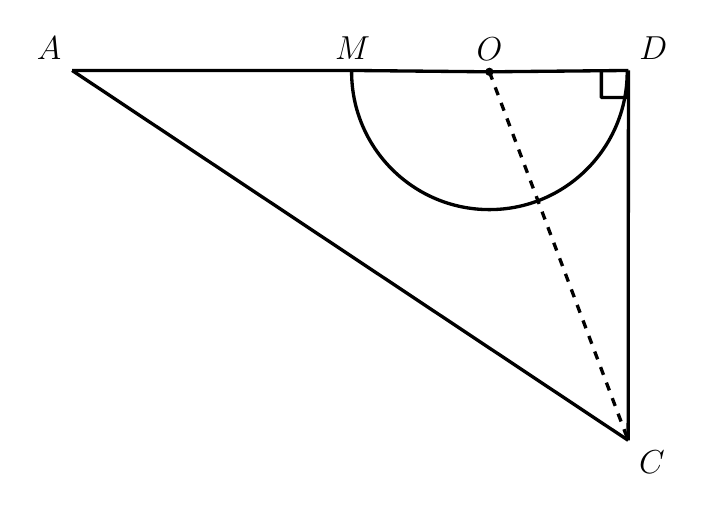
\begin{tikzpicture}[line width=1.2pt, line join=round]
\coordinate (A) at (-3.559,2.221);
\coordinate (C) at (3.502,-2.476);
\coordinate (D) at (3.506,2.221);
\coordinate (M) at (0.001,2.221);
\coordinate (O) at (1.740,2.204);









\draw (A) -- (M) -- (O) -- (D);
\draw (A) -- (C);
\draw (C) -- (D);


\draw[dashed] (O) -- (C);


\draw ($(O)+(180.000:1.750)$) arc[start angle=180.000, end angle=360.000, radius=1.750];


\draw pic[draw, angle radius=0.344cm] {right angle=A--D--C};

\fill (O) circle (1.500pt);


\node[above left, font=\fontsize{12.5}{15}\selectfont] at (A) {$A$};
\node[above, font=\fontsize{12.5}{15}\selectfont] at (M) {$M$};
\node[above, font=\fontsize{12.5}{15}\selectfont] at (O) {$O$};
\node[above right, font=\fontsize{12.5}{15}\selectfont] at (D) {$D$};
\node[below right, font=\fontsize{12.5}{15}\selectfont] at (C) {$C$};
\end{tikzpicture}
\end{document}